\section{Laboratory :Silicon Synapses }

In this session, we study how synaptic circuits generate current when stimulated by voltage pulses. Specifically we will measure the response of a synapse to a single pulse, and to a sequence of spikes.

To this extend, we will measure the response properties of the diff-pair integrator (DPI) synapse . 

\subsection{DPI synapse}

The DPI synapse receives a voltage pulse train, $V_{pulse}$, as input and outputs a corresponding synaptic current, $I_{syn}$ and voltage $V_{syn}$. 
Bias parameters $V_{weight}$ & $V_{tau}$ affect the amplitude and decay of the response, while $V_{thr}$ acts as an additional weight bias. $C_{syn}$ sizing was chosen for a capacitance of 2pF. 


We need to tune these parameters and observe the behavior of the DPI synapse. 
To test the basic response of the circuit we send 2 input pulses and sample 10 points, with a delta t of 0.02 between the samples. 


\begin{figure}[H]
    \centering
    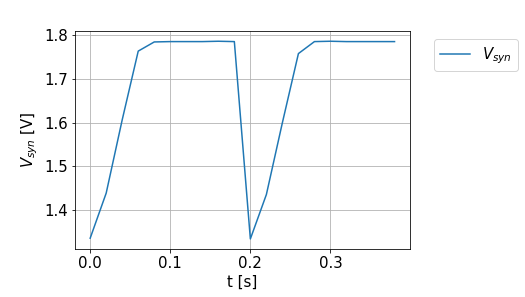
\includegraphics[width=0.95\linewidth]{Figures/synapse_lab.png}
    \caption{Measured values of $V_{syn}$ as a function of time}
    \label{fig:basalandcerebellum}
\end{figure}

\begin{figure}[H]
    \centering
    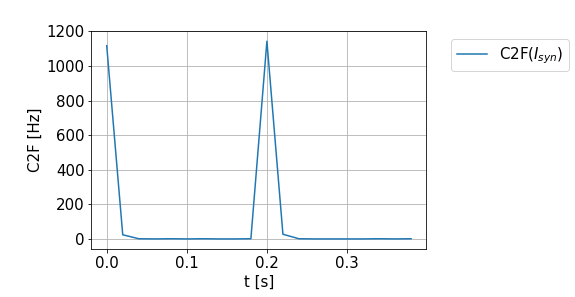
\includegraphics[width=0.95\linewidth]{Figures/synapse_current.png}
    \caption{Measured C2F values of $I_{syn}$ as a function of time}
    \label{fig:basalandcerebellum}
\end{figure}


We found that if we increase $V_{weight}$ or $V_{thr}$ the amplitude of $I_{syn}$ increases and $V_{syn}$ will need more time to recharge and return back to it's initial state (1.8V). 

With a larger $V_{tau}$ or $V_{pulse}$ the opposite is truth. The amplitude of $I_{syn}$ shrinks and $V_{syn}$ returns to the pre-spike state much faster. 




